\section{Single Page Applikation}

\paragraph{Spørgsmål}
Redegør for og vis eksampler på hvordan man kan designe	og implementere Single-page applikationer med brug af	Angular2 eller nyere.

\subsection{Angular}
Open-source javascript client side MVC framework. Udviklet og vedligeholdt af Google.

\paragraph{Sprog} Man er ikke låst til ét sprog.

\begin{multicols}{5}
	\begin{itemize}
		\item JavaScript
		\item Dart
		\item TypeScript
	\end{itemize}
\end{multicols}

\subsubsection{Framework}
Første request svarer med \textit{Index.html} og herefter hentes øvrigt indhold som AJAX requests. Komponenter skiftes ud med javascript. Figur~\ref{fig:ng-basics} viser et generelt flow for en angular app.

\begin{figure}[H]
	\centering
	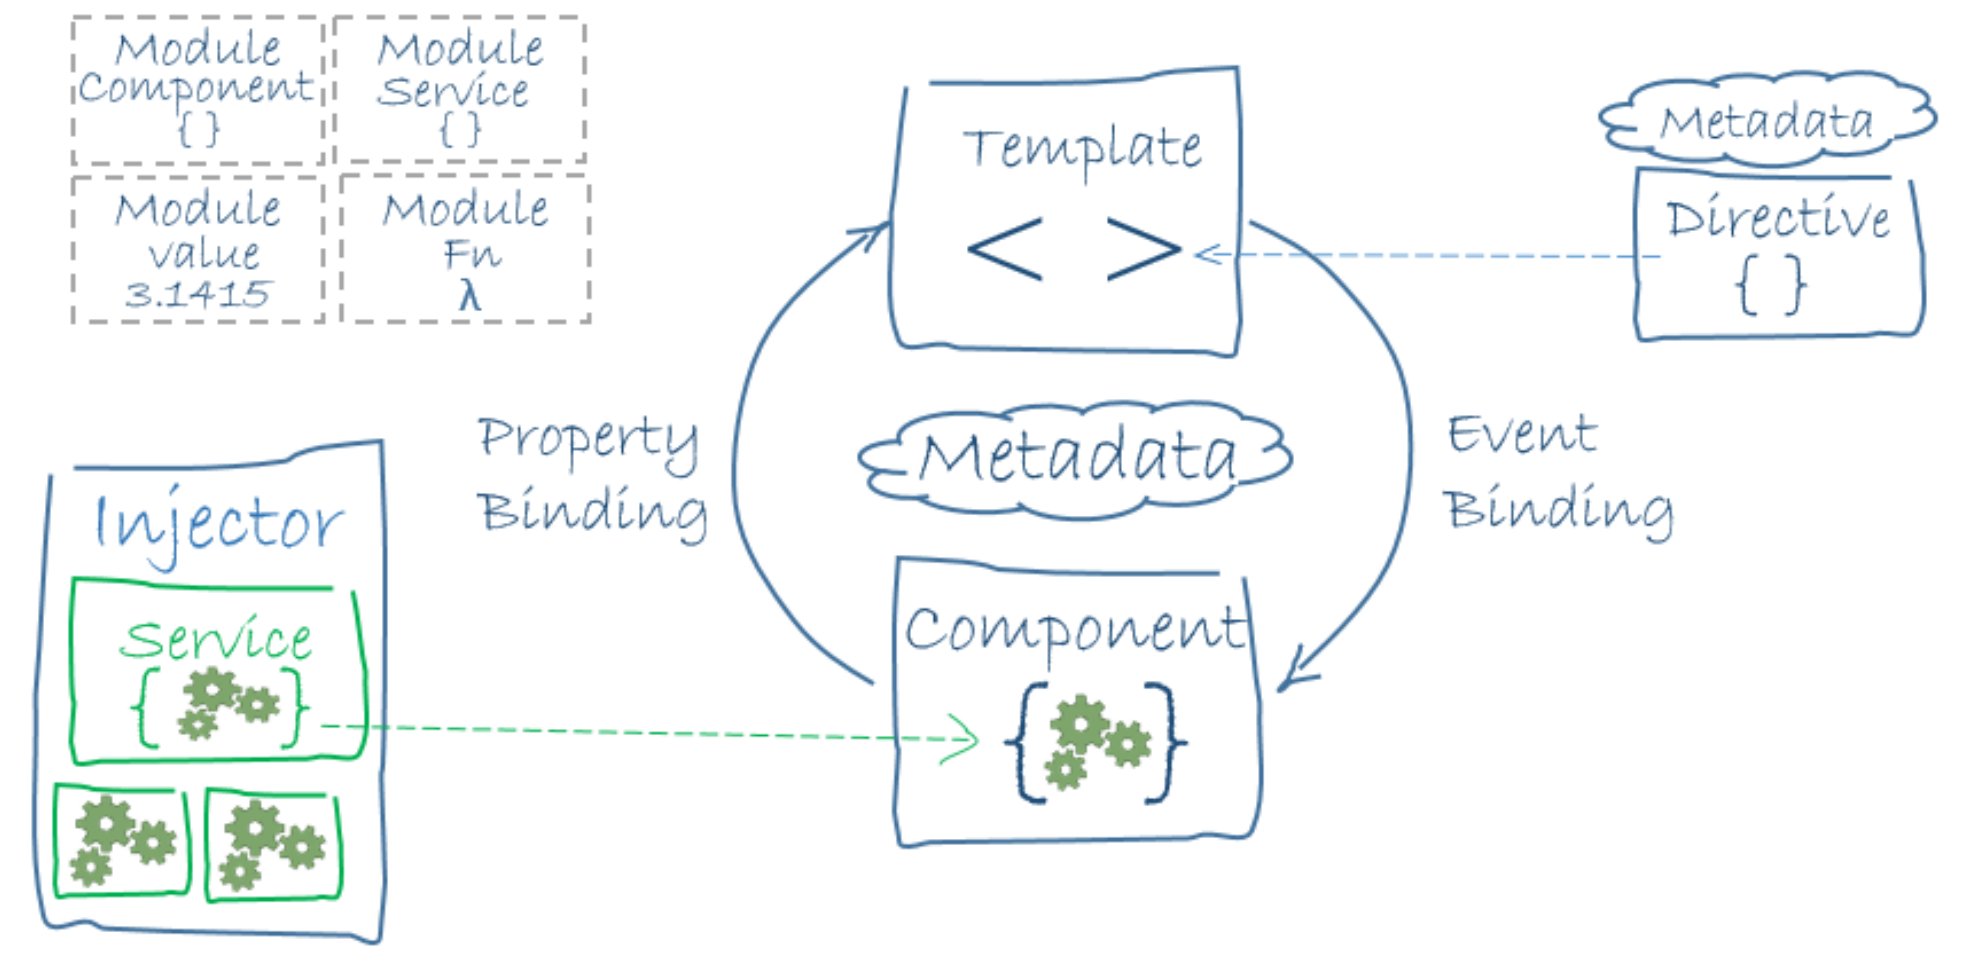
\includegraphics[width=\linewidth]{figs/ng-basics}
	\caption{Basale byggeblokke i Angular.}
	\label{fig:ng-basics}
\end{figure}

Angular er et komplet framework, so giver adgang til følgende features for at gøre udvikling så let som mulig.

\begin{multicols}{2}
\paragraph{Module} organiserer koden.
\paragraph{Component} giver UI widgets.
\paragraph{Pipe} formatere data.
\paragraph{Directive} manipulere DOM.
\paragraph{HTTP Module} til netværkskald.
\paragraph{CLI} til tooling og scaffolding.
\paragraph{Routing} i flere lag.
\paragraph{Forms} dynamiske og reaktive.
\paragraph{Injectable} services og delt logik.
\paragraph{Binding} to- og en-vejs. 
\end{multicols}
